\documentclass[letterpaper, 12pt]{artikel3}

\usepackage{geometry}
\geometry{left=3cm,right=3cm,top=4cm,bottom=4cm}
\usepackage[fleqn]{amsmath}

% These packages add a few useful math symbols.
\usepackage{amssymb}
\usepackage{amsmath}
\usepackage{mathtools}
\usepackage{listings}
\usepackage{amsmath}
\usepackage{amssymb}
\lstset{language=Matlab}
\usepackage{euler}


%Karnaugh map
\usepackage{tikz}
\usepackage{askmaps}
\usepackage{circuitikz}
\usetikzlibrary{matrix,calc}
\usetikzlibrary{automata,positioning}
\usepackage{amssymb}
\usepackage{tikz}


\usetikzlibrary{circuits.logic.US,circuits.logic.IEC}

% The verbatim package allows pre-formatted text (like code) to be included.
\usepackage{verbatim}

% The algorithmic package provides a somewhat convenient way to typeset
% algorithms.
\usepackage{algorithm}
\usepackage[noend]{algpseudocode}

\usepackage{float}

\makeatletter
\def\BState{\State\hskip-\ALG@thistlm}
\makeatother

\usepackage{fancyhdr}
\pagestyle{fancy}
\lhead{}
\chead{CSC421 Artificial Intelligence  Assignment \#3 | YUE LYU V00902738}
\rhead{}
\renewcommand{\headrulewidth}{0.4pt}

%  \quad & (p \lor q \lor \urcorner r) \land (( r \land \urcorner q \land \urcorner p) \lor ((r \land  \urcorner q  \land \urcorner p )) 
\begin{document}

\section*{Question 1}
 $(p | q | -r) \& ((-r | q | p) -> ((r | q) \& -q \& -p))$
\begin{align*}
  &(p \lor q \lor \urcorner r) \land ((\urcorner r \lor q \lor p) \Rightarrow  ((r \lor q) \land \urcorner q \land \urcorner p)) \\
I \quad & (p \lor q \lor \urcorner r) \land ( \urcorner (\urcorner r \lor q \lor p) \lor  ((r \lor q) \land \urcorner q \land \urcorner p) )   \\
N \quad & (p \lor q \lor \urcorner r) \land (( r \land \urcorner q \land \urcorner p) \lor  ((r \lor q) \land \urcorner q \land \urcorner p) )   \\
 D \quad& (p \lor q \lor \urcorner r) \land ((   (r \land \urcorner q \land \urcorner p) \lor  (r \lor q))  \land ((  (r \land \urcorner q \land \urcorner p) \lor \urcorner q)) \land (( (r \land \urcorner q \land \urcorner p) \lor \urcorner p) ))\\ 
 D \quad& (p \lor q \lor \urcorner r) \land (( (r \lor r \lor q ) \land (\urcorner q \lor r \lor q) \land (\urcorner p \lor r \lor q) \\ & \land (r \lor  \urcorner q ) \land (\urcorner q \lor \urcorner q) \land (\urcorner p \lor \urcorner q) \land (r \lor  \urcorner p ) \land (\urcorner q \lor \urcorner p) \land (\urcorner p \lor \urcorner p))) \\
O \quad &\\
1\quad &  \{p, q, \urcorner r\}\\
2\quad &   \{r, q\} \\
3\quad &   \{\urcorner q, r, q\} \\
4\quad &   \{\urcorner p, r, q\}  \\
5\quad &   \{r, \urcorner q\} \\
6\quad &   \{\urcorner q\} \\
7\quad &   \{\urcorner p, \urcorner q\} \\
8\quad &   \{r, \urcorner p\} \\
9\quad &   \{\urcorner q, \urcorner p\} \\
10\quad &   \{\urcorner p\} \\
Resolution \\
11 \quad &  \{p, q\}  & 1,2\\
12 \quad &  \{p\}  & 6, 11\\
13 \quad &  \{\}  &	10,12\\
\end{align*}
\section*{Question 2}

$\forall x \forall y (Horse(x) \land Dog(y) \Rightarrow Faster(x,y))$\\
$\exists g (Greyhound(g) \land \forall r (Rabbit(r) \Rightarrow Faster(g,r)))$\\
$\forall x  \forall r  (Horse(x) \land Rabbit(r) \Rightarrow  Faster(x,r))$\\
neg conclusion: $ \urcorner (\forall x  \forall r  (Horse(x) \land Rabbit(r) \Rightarrow  Faster(x,r)))$\\
Now turn them to clausal form and do the resolution steps.\\
\begin{align*}
&\forall x \forall y (Horse(x) \land Dog(y) \Rightarrow Faster(x,y))\\
I \quad & \forall x \forall y  (\urcorner ((Horse(x) \land Dog(y))  \lor Faster(x,y) )\\
N \quad & \forall x \forall y (\urcorner Horse(x) \lor \urcorner Dog(y) \lor Faster(x,y)) \\
E \quad & \urcorner Horse(x) \lor \urcorner Dog(y) \lor Faster(x,y)\\
O \quad & \{ \urcorner Horse(x), \urcorner Dog(y), Faster(x,y) \}\\
\end{align*}

\begin{align*}
& \exists g (Greyhound(g) \land \forall r (Rabbit(r) \Rightarrow Faster(g,r)))\\
I \quad & \exists g (Greyhound(g) \land \forall r (\urcorner Rabbit(r) \lor  Faster(g,r)))\\
E \quad &  \exists g (Greyhound(g) \land (\urcorner Rabbit(r) \lor  Faster(g,r)))\\
A \quad &  Greyhound(Grey) \land (\urcorner Rabbit(r) \lor  Faster(Grey,r)))\\
O \quad & \{Greyhound(Grey)\}\\
\quad & \{\urcorner Rabbit(r),Faster(Grey,r)\}\\
\end{align*}

Conclusion:\\
\begin{align*}
&\urcorner (\forall x  \forall r  (Horse(x) \land Rabbit(r) \Rightarrow  Faster(x,r)))\\
I \quad & \urcorner (\forall x  \forall r  (\urcorner ((Horse(x) \land Rabbit(r)) \lor Faster(x,r)))\\
N \quad & \urcorner (\forall x  \forall r ( \urcorner Horse(x) \lor \urcorner Rabbit(r) \lor Faster(x,r)))\\
N \quad & \exists x \exists r \urcorner ( \urcorner Horse(x) \lor \urcorner Rabbit(r) \lor Faster(x,r)))\\
N \quad & \exists x \exists r (Horse(x) \land  Rabbit(r) \land \urcorner Faster(x,r)) \\
A \quad & Horse(Happy) \land  Rabbit(Rein) \land \urcorner Faster(Happy,Rein)\\
O \quad & \{Horse(Happy)\} \\
\quad & \{Rabbit(Rein)\}\\
\quad & \{\urcorner Faster(Happy,Rein)\}\\
\end{align*}
And the backgroud knowledge:\\
$\forall g (Greyghound(g) \Rightarrow Dog(g))$\\
$\forall x \forall y \forall z(Faster(x,y) \land Faster(y,z) \Rightarrow Faster(x,z))$\\

\begin{align*}
& \forall g (Greyghound(g) \Rightarrow Dog(g))\\
I \quad & \forall g \urcorner Greyghound(g) \lor Dog(g)) \\
A \quad & \urcorner Greyghound(g) \lor Dog(g)) \\
O \quad & \{ \urcorner Greyghound(g), Dog(g) \}\\
\end{align*}

\begin{align*}
&\forall x \forall y \forall z (Faster(x,y) \land Faster(y,z) \Rightarrow Faster(x,z))\\
I \quad & x \forall y \forall z( \urcorner (Faster(x,y) \land Faster(y,z) ) \lor Faster(x,z) ) \\ 
N \quad & \forall y \forall z (\urcorner Faster(x,y) \lor \urcorner Faster(y,z)  \lor Faster(x,z) ) \\ 
A \quad & \urcorner Faster(x,y) \lor \urcorner Faster(y,z)  \lor Faster(x,z)\\
O \quad & \{ \urcorner Faster(x,y), \urcorner Faster(y,z), Faster(x,z) \}\\
\end{align*}

Resolution: 
\begin{align*}
1 \quad & \{ \urcorner Horse(x_1), \urcorner Dog(y_1), Faster(x_1,y_1) \}\\
2 \quad & \{Greyhound(Grey)\}\\
3 \quad & \{\urcorner Rabbit(r_1),Faster(Grey,r_1)\} \\
4 \quad & \{ \urcorner Greyghound(g_1), Dog(g_1) \} \\
5 \quad & \{ \urcorner Faster(x_2,y_2), \urcorner Faster(y_2,z_1), Faster(x_2,z_1) \} \\
6 \quad &  \{Horse(Happy)\} \\
7 \quad & \{Rabbit(Rein)\}\\
8 \quad & \{\urcorner Faster(Happy,Rein)\}\\
9 \quad & \{Dog(Grey) \} & 2,4\\ 
10 \quad & \{Faster(Grey, Rein)\} & 3,7\\
11 \quad & \{\urcorner Horse(x_1), Faster(x_1,Grey)\} & 1,9\\
12 \quad & \{Faster(Happy,Grey)\} & 6,11\\
13 \quad & \{\urcorner Faster(Grey,z_1), Faster(Happy,z_1) \} & 5,12\\
14 \quad & \{ Faster(Happy,Rein) \} & 10,13\\
15 \quad & \{ \} & 8,14\\
\end{align*}
\section*{Question 3}
$\forall x (Hummingbird(x) \Rightarrow Richcolor(x) )$ \\ 
$\urcorner \exists y ( Bird(y) \land Large(y) \land LiveonHon(y))$\\
$\forall y (Bird(y) \land \urcorner LiveonHon(y) \Rightarrow \urcorner Richcolor(y))$\\
$\forall x (Hummingbird(x) \Rightarrow Bird(x) )$  (Background)\\\
$\forall x (Hummingbird(x) \Rightarrow \urcorner Large(x))$  (Conlusion)\\

Prover 9:\\
%\begin{align*}
%& \quad all x (hummingbird(x) -> richcolor(x)).\\
%& \quad all y -(bird(y) \& large(y) -> liveonhon(y)).\\
%& \quad all y (bird(y) \& - liveonhon(y) -> dullcolor(y)).\\
%& \quad all x (hummingbird(x) -> bird(x)).\\
%& \quad all y -(bird(y) \& large(y) -> small(y)).\\
%& \quad all y -(bird(y) \& richcolor(y) -> dullcolor(y)).\\
%& \quad all x (hummingbird(x) -> small(x)).  (Conlusion)\\
%\end{align*}

%\begin{align*}
%1 & \quad (all x (hummingbird(x) -> richcolor(x))) [assumption].\\
%2 & \quad (all x -(bird(x) \& large(x) -> liveonhon(x)))   [assumption]. \\
%3 & \quad (all x (bird(x) \& -liveonhon(x) -> dullcolor(x)))  [assumption]. \\
%4 & \quad (all x (hummingbird(x) -> bird(x)))  [assumption].\\
%5 & \quad (all y -(bird(y) \& large(y) -> small(y))) [assumption].\\
%6 & \quad (all x -(bird(x) \& richcolor(x) -> dullcolor(x)))  [assumption]. \\
%11& \quad -bird(x) | liveonhon(x) | dullcolor(x).  [clausify(3)].\\
%12& \quad bird(x).  [clausify(2)].\\
%16& \quad liveonhon(x) | dullcolor(x).  [resolve(11,a,12,a)].\\
%17& \quad -liveonhon(x).  [clausify(2)].\\
%18& \quad dullcolor(x).  [resolve(16,a,17,a)].\\
%19& \quad -dullcolor(x).  [clausify(6)].\\
%20& \quad \$F.  [resolve(18,a,19,a)].\\
%\end{align*}

\begin{align*}
1& (all x (hummingbird(x) -> richcolor(x)))   [assumption]. \\
2& (all x -(bird(x) \& large(x) \& liveonhon(x)))  [assumption].\\
3& (all x (bird(x) \& -liveonhon(x) -> -richcolor(x)))  [assumption].\\
4& (all x (hummingbird(x) -> bird(x)))   [assumption].\\
5& (all x (hummingbird(x) -> -large(x)))   [goal].\\
6& hummingbird(c1).  [deny(5)].\\
7& -hummingbird(x) | richcolor(x).  [clausify(1)].\\
8& -hummingbird(x) | bird(x).  [clausify(4)].\\
9& bird(c1).  [resolve(6,a,8,a)].\\
10& -bird(x) | -large(x) | -liveonhon(x).  [clausify(2)].\\
11& -bird(x) | liveonhon(x) | -richcolor(x).  [clausify(3)].\\
12& -large(c1) | -liveonhon(c1).  [resolve(9,a,10,a)].\\
13& large(c1).  [deny(5)].\\
14& liveonhon(c1) | -richcolor(c1).  [resolve(9,a,11,a)].\\
15& richcolor(c1).  [resolve(6,a,7,a)].\\
16& liveonhon(c1).  [resolve(14,b,15,a)].\\
17& -liveonhon(c1).  [resolve(12,a,13,a)].\\
18& \$F.  [resolve(16,a,17,a)].
\end{align*}


\section*{Question 4}
mg = My gardener; wl = worth listening to on military subjects; \\
ar = able to remember the battle of waterloo; old=very old \\
\begin{align*}
& \exists x (person(x) \land mg(x) \land wl(x)). \\
& \forall y ( (person(y) \land ar(y)) \Rightarrow old(y) ). \\
& \forall z ( (person(z) \land wl(z)) \Rightarrow ar(z) ). \\
& \exists m (person(x) \land mg(m) \land old(m)).  (conclusion)\\
\end{align*}

Prover 9:\\
\begin{align*}
1 &(exists x (person(x) \& mg(x) \& wl(x)))  [assumption].\\
2 &(all x (person(x) \& ar(x) -> old(x)))  [assumption].\\
3 &(all x (person(x) \& wl(x) -> ar(x))) [assumption].\\
4 &(exists m (person(m) \& mg(m) \& old(m)))  [goal].\\
5 &-person(x) | -ar(x) | old(x).  [clausify(2)].\\
6 &person(c1).  [clausify(1)].\\
7 &-person(x) | -wl(x) | ar(x).  [clausify(3)].\\
8 &-person(x) | -mg(x) | -old(x).  [deny(4)].\\
9 &-mg(c1) | -old(c1).  [resolve(8,a,6,a)].\\
10 &mg(c1).  [clausify(1)].\\
11 &-wl(c1) | ar(c1).  [resolve(7,a,6,a)].\\
12 &wl(c1).  [clausify(1)].\\
13 &ar(c1).  [resolve(11,a,12,a)].\\
14 &-ar(c1) | old(c1).  [resolve(5,a,6,a)].\\
15 &old(c1).  [resolve(13,a,14,a)].\\
16 &-old(c1).  [resolve(9,a,10,a)].\\
17 &\$F.  [resolve(15,a,16,a)].
\end{align*}

\section*{Question 5}
$P(P_{13}) = P(P_{22}) = P(P_{31}) = 0.01$
\begin{align*}
P(p_{13}| b_{12},b_{21}) &=\alpha \sum_{p_{22}} \sum_{p_{31}}(P(b_{12}|p_{13},p_{22}) \cdot P(b_{21}|p_{22},p_{31})\cdot P(p_{13}) \cdot P(p_{22}) \cdot P(p_{31}) )  \\
&=  \alpha[ P(b_{12}|p_{13},p_{22}) \cdot P(b_{21}|p_{22},p_{31})\cdot  P(p_{13}) \cdot P(p_{22}) \cdot P(p_{31})  +  \\
\quad & P(b_{12}|p_{13},\urcorner p_{22}) \cdot P(b_{21}|\urcorner  p_{22},p_{31})\cdot  P(p_{13}) \cdot P( \urcorner p_{22}) \cdot P(p_{31})  + \\
\quad& P(b_{12}|p_{13},p_{22}) \cdot P(b_{21}|p_{22},\urcorner p_{31})\cdot  P(p_{13}) \cdot P(p_{22}) \cdot P(\urcorner p_{31}) +\\
\quad& P(b_{12} p_{13},p_{22}) \cdot P(b_{21}|\urcorner p_{22},\urcorner p_{31})\cdot  P(p_{13}) \cdot P(\urcorner p_{22}) \cdot P(\urcorner p_{31}) ] \\
&= \alpha [1 \cdot 1  \cdot 0.01 \cdot 0.01 \cdot 0.01 + 1 \cdot 1 \cdot 0.01 \cdot 0.99 \cdot 0.01 + \\
& 1 \cdot 1 \cdot 0.01 \cdot 0.01 \cdot 0.99 + 0]  = \alpha (0.000001 + 0.000099 + 0.000099) \\ 
&= 0.000199 \alpha \\
\\
P(\urcorner p_{13}| b_{12},b_{21}) &=\alpha \sum_{p_{22}} \sum_{p_{31}}(P(b_{12}|\urcorner p_{13},p_{22}) \cdot P(b_{21}|p_{22},p_{31})\cdot P(\urcorner  p_{13}) \cdot P(p_{22}) \cdot P(p_{31}) ) \\ 
&=  \alpha[ P(b_{12}|\urcorner p_{13},p_{22}) \cdot P(b_{21}|p_{22},p_{31})\cdot  P(\urcorner p_{13}) \cdot P(p_{22}) \cdot P(p_{31}) +  \\
\quad & P(b_{12}|\urcorner p_{13},\urcorner p_{22}) \cdot P(b_{21}|\urcorner  p_{22},p_{31})\cdot  P(\urcorner p_{13}) \cdot P( \urcorner p_{22}) \cdot P(p_{31})  + \\
\quad& P(b_{12}|\urcorner p_{13},p_{22}) \cdot P(b_{21}|p_{22},\urcorner p_{31})\cdot  P(\urcorner p_{13}) \cdot P(p_{22}) \cdot P(\urcorner p_{31}) +\\
\quad& P(b_{12} |\urcorner p_{13},p_{22}) \cdot P(b_{21}|\urcorner p_{22},\urcorner p_{31})\cdot  P(\urcorner p_{13}) \cdot P(\urcorner p_{22}) \cdot P(\urcorner p_{31}) ] \\
& = \alpha [1 \cdot 1  \cdot 0.99 \cdot 0.01 \cdot 0.01 + 0 + 1\cdot 1\cdot 0.99 \cdot 0.01 \cdot 0.99 + 0)   \\
& =\alpha (0.000099 + 0.009801) =  0.0099\alpha  \\
\\
\alpha &= 1/(0.000199 +0.0099) = 99.02\\
P( p_{13}| b_{12},b_{21}) &= 0.0197\\
P(\urcorner p_{13}| b_{12},b_{21}) &= 0.9803\\
\\
P(p_{31}| b_{12},b_{21}) &=\alpha \sum_{p_{13}} \sum_{p_{22}}(P(b_{12}|p_{13},p_{22}) \cdot P(b_{21}|p_{22},p_{31})\cdot P(p_{13}) \cdot P(p_{22}) \cdot P(p_{31}) )  \\
&=  0.0197\\
P(\urcorner p_{31}| b_{12},b_{21}) &=\alpha \sum_{p_{13}} \sum_{p_{22}}(P(b_{12}|p_{13},p_{22}) \cdot P(b_{21}|p_{22},\urcorner p_{31})\cdot P(p_{13}) \cdot P(p_{22}) \cdot P ( \urcorner p_{31}) ) \\
&= 0.9803 \\
\end{align*}

\begin{align*}
P(p_{22}| b_{12},b_{21}) &=\alpha \sum_{p_{13}} \sum_{p_{31}}(P(b_{12}|p_{13},p_{22}) \cdot P(b_{21}|p_{22},p_{31})\cdot P(p_{13}) \cdot P(p_{22}) \cdot P(p_{31}) )  \\ 
&=  \alpha[ P(b_{12}|p_{13},p_{22}) \cdot P(b_{21}|p_{22},p_{31})\cdot  P(p_{13}) \cdot P(p_{22}) \cdot P(p_{31})  +  \\
\quad & P(b_{12}|\urcorner p_{13},p_{22}) \cdot P(b_{21}| p_{22},p_{31})\cdot  P(\urcorner p_{13}) \cdot P( p_{22}) \cdot P(p_{31})  + \\
\quad& P(b_{12}|p_{13},p_{22}) \cdot P(b_{21}|p_{22},\urcorner p_{31})\cdot  P(p_{13}) \cdot P(p_{22}) \cdot P(\urcorner p_{31}) +\\
\quad& P(b_{12} |\urcorner p_{13},p_{22}) \cdot P(b_{21}| p_{22},\urcorner p_{31})\cdot  P( \urcorner p_{13}) \cdot P( p_{22}) \cdot P(\urcorner p_{31}) ] \\
& = \alpha( 1 \cdot 1\cdot 0.01 \cdot 0.01 \cdot 0.01 
+ 1 \cdot 1\cdot 0.01 \cdot 0.01 \cdot 0.99 \\
& + 1 \cdot 1\cdot 0.01 \cdot 0.01 \cdot 0.99
+  1 \cdot 1 \cdot 0.99 \cdot 0.01 \cdot 0.99) \\
& = 0.01 \alpha \\
\\
P(\urcorner p_{22}| b_{12},b_{21}) &=\alpha \sum_{p_{13}} \sum_{p_{31}}(P(b_{12}|p_{13},\urcorner  p_{22}) \cdot P(b_{21}| \urcorner p_{22},p_{31})\cdot P(p_{13}) \cdot P(\urcorner  p_{22}) \cdot P(p_{31}) )  \\
&=  \alpha[ P(b_{12}|p_{13},\urcorner p_{22}) \cdot P(b_{21}|\urcorner p_{22},p_{31})\cdot  P(p_{13}) \cdot P(\urcorner p_{22}) \cdot P(p_{31})  +  \\
\quad & P(b_{12}|\urcorner p_{13},\urcorner p_{22}) \cdot P(b_{21}| \urcorner p_{22},p_{31})\cdot  P(\urcorner p_{13}) \cdot P(\urcorner p_{22}) \cdot P(p_{31})  + \\
\quad& P(b_{12}|p_{13},\urcorner p_{22}) \cdot P(b_{21}|\urcorner p_{22},\urcorner p_{31})\cdot  P(p_{13}) \cdot P(\urcorner p_{22}) \cdot P(\urcorner p_{31}) +\\
\quad& P(b_{12} |\urcorner p_{13},\urcorner p_{22}) \cdot P(b_{21}| \urcorner p_{22},\urcorner p_{31})\cdot  P( \urcorner p_{13}) \cdot P(\urcorner  p_{22}) \cdot P(\urcorner p_{31}) ] \\ 
& = \alpha( 1 \cdot 1  \cdot 0.01\cdot 0.99 \cdot 0.01 + 0 + 0+0) = 0.000099 \alpha \\
\\
\alpha & = 1/(0.01 + 0.000099) = 99.02\\
P(p_{22}| b_{12},b_{21}) &= 0.9902\\
P(\urcorner p_{22}| b_{12},b_{21}) &=0.0098 \\
\end{align*}
Going to [2,2] is almost certain death. So, a probabilistic agent will never choose to go to [2,2].
On the other hand, to a logical agent, squares [1,3], [2,2], [3,1] look the same. So, the logical agent would choose either one with equal chance (1/3). By doing that, the agent will die with a chance of about 1/3.

\section*{Question 6}
\subsection*{1} %1. (1 pt) Draw the Bayesian network.
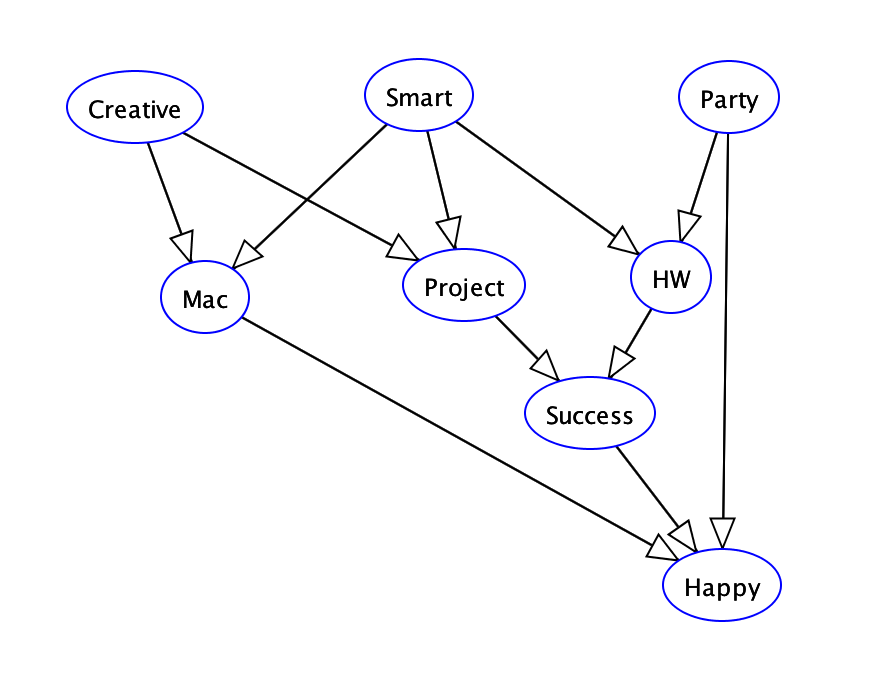
\includegraphics[scale=0.6]{QQ20191109-1232162x.png}
\subsection*{2}%2. (2 pt) Estimate the probabilities of the conditional probability tables using the data provided (you can use Excel pivot tables for counting).
%$P(party)= 0.6022, P(smart) = 0.7048,  P(creative) = 0.6994$\\
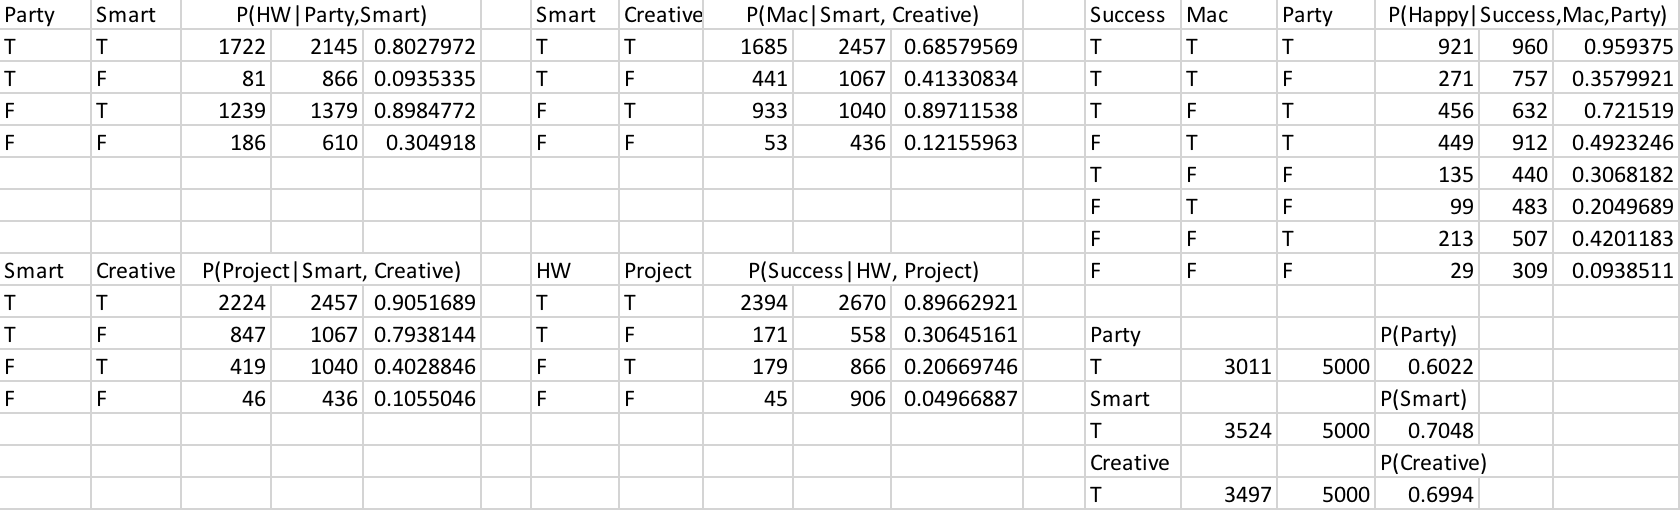
\includegraphics[scale=0.5]{QQ20191100.png}
\subsection*{3}%3. (2 pts) What is the probability of being happy given that you party often, are wicked smart, but not very creative? Show details of computation.
\begin{align*}
&P(happy| party, smart, \urcorner creative) \\
& = \alpha\sum_{mac} \sum_{project} \sum_{hw} \sum_{success} [P(happy, mac, success, hw, project,party,smart, \urcorner  creative) ] \\
& = \alpha\sum_{mac} \sum_{project} \sum_{hw} \sum_{success} [P(happy |mac, success, party)\cdot P(mac| \urcorner creative, smart) \cdot \\
& P(success | project, hw) \cdot P(hw| party, smart) \cdot P(project|\urcorner  creative, smart) \cdot \\
& P(party)\cdot P(smart) \cdot  P(\urcorner creative)]\\
& = \alpha  P(party)\cdot P(smart) \cdot  P(\urcorner creative)   \cdot \sum_{project}  \cdot  P(project|\urcorner  creative, smart) \\
& \sum_{mac}\sum_{hw} \sum_{success} P(happy |mac, success, party) \cdot P(mac| \urcorner creative, smart) \cdot \\
& P(success | project, hw) \cdot P(hw| party, smart) \\
& = \alpha  P(party)\cdot P(smart) \cdot  P(\urcorner creative)   \cdot \sum_{project}  \cdot  P(project|\urcorner  creative, smart)  \\
& [P(happy |mac, success, party) \cdot P(mac| \urcorner creative, smart) \cdot \\
& P(success | project, hw) \cdot P(hw| party, smart) +\\
& P(happy |\urcorner mac, success, party) \cdot P( \urcorner mac| \urcorner creative, smart) \cdot \\
& P(success | project, hw) \cdot P(hw| party, smart)  +\\
& P(happy |mac, success, party) \cdot P(mac| \urcorner creative, smart) \cdot \\
& P(success | project, \urcorner hw) \cdot P(\urcorner hw| party, smart) +\\
& P(happy |mac,\urcorner success, party) \cdot P(mac| \urcorner creative, smart) \cdot \\
& P(\urcorner success | project, hw) \cdot P(hw| party, smart) +\\
& P(happy |\urcorner mac,\urcorner success, party) \cdot P(\urcorner mac| \urcorner creative, smart) \cdot \\
& P(\urcorner success | project, hw) \cdot P(hw| party, smart) +\\
& P(happy |\urcorner mac, success, party) \cdot P(\urcorner mac| \urcorner creative, smart) \cdot \\
& P(success | project,\urcorner hw) \cdot P(\urcorner hw| party, smart) +\\
& P(happy |mac,\urcorner success, party) \cdot P(mac| \urcorner creative, smart) \cdot \\
& P(\urcorner success | project,\urcorner hw) \cdot P(\urcorner hw| party, smart) +\\
& P(happy |\urcorner mac, \urcorner success, party) \cdot P(\urcorner mac| \urcorner creative, smart) \cdot \\
& P(\urcorner success | project, \urcorner hw) \cdot P(\urcorner hw| party, smart) ]\\
& = 0.692
\end{align*}
%& = \alpha *0.6022 * 0.7048 * 0.3006 *[0.35795 *0.14171* 0.85837*  0.53346 +  \\ 
%& = 0.17723* (1-0.14171)*0.85837* 0.53346  + \\
%& = 0.35795* 0.14171*0.06418071 *(1-0.53346) + \\
%& = 0.174504469* 0.14171* (1-0.858372176)*0.53346 +\\
%& = 0.17723*(1-0.141709512) *0.06418071 *(1-0.533457249) + \\
%& = 0.174504469* 0.141709512*(1-0.06418071) *(1-0.533457249) +\\
%& = 0.082782744*(1-0.141709512) * (1-0.858372176)* 0.533457249 + \\
%& = 0.082782744* (1-0.141709512)*(1-0.06418071)* (1-0.533457249) ]\\
%& = 0.01888361414656664 \alpha\\

\begin{align*}
&P(\urcorner happy| party, smart, \urcorner creative) \\
& = \alpha\sum_{mac} \sum_{project} \sum_{hw} \sum_{success} [P(\urcorner happy, mac, success, hw, project,party,smart, \urcorner  creative) ] \\
& = \alpha\sum_{mac} \sum_{project} \sum_{hw} \sum_{success} [P(\urcorner happy |mac, success, party)\cdot P(mac| \urcorner creative, smart) \cdot \\
& P(success | project, hw) \cdot P(hw| party, smart) \cdot P(project|\urcorner  creative, smart) \cdot \\
& P(party)\cdot P(smart) \cdot  P(\urcorner creative)]\\
& = \alpha  P(party)\cdot P(smart) \cdot  P(\urcorner creative)   \cdot \sum_{project}  \cdot  P(project|\urcorner  creative, smart) \\
& \sum_{mac}\sum_{hw} \sum_{success} P(\urcorner happy |mac, success, party) \cdot P(mac| \urcorner creative, smart) \cdot \\
& P(success | project, hw) \cdot P(hw| party, smart) \\
& = \alpha  P(party)\cdot P(smart) \cdot  P(\urcorner creative)   \cdot \sum_{project}  \cdot  P(project|\urcorner  creative, smart)  \\
& [P(\urcorner happy |mac, success, party) \cdot P(mac| \urcorner creative, smart) \cdot \\
& P(success | project, hw) \cdot P(hw| party, smart) +\\
& P(\urcorner happy |\urcorner mac, success, party) \cdot P( \urcorner mac| \urcorner creative, smart) \cdot \\
& P(success | project, hw) \cdot P(hw| party, smart)  +\\
& P(\urcorner happy |mac, success, party) \cdot P(mac| \urcorner creative, smart) \cdot \\
& P(success | project, \urcorner hw) \cdot P(\urcorner hw| party, smart) +\\
& P(\urcorner happy |mac,\urcorner success, party) \cdot P(mac| \urcorner creative, smart) \cdot \\
& P(\urcorner success | project, hw) \cdot P(hw| party, smart) +\\
& P(\urcorner happy |\urcorner mac,\urcorner success, party) \cdot P(\urcorner mac| \urcorner creative, smart) \cdot \\
& P(\urcorner success | project, hw) \cdot P(hw| party, smart) +\\
& P(\urcorner happy |\urcorner mac, success, party) \cdot P(\urcorner mac| \urcorner creative, smart) \cdot \\
& P(success | project,\urcorner hw) \cdot P(\urcorner hw| party, smart) +\\
& P(\urcorner happy |mac,\urcorner success, party) \cdot P(mac| \urcorner creative, smart) \cdot \\
& P(\urcorner success | project,\urcorner hw) \cdot P(\urcorner hw| party, smart) +\\
& P(\urcorner happy |\urcorner mac, \urcorner success, party) \cdot P(\urcorner mac| \urcorner creative, smart) \cdot \\
& P(\urcorner success | project, \urcorner hw) \cdot P(\urcorner hw| party, smart) ]\\
& = 0.308
\end{align*}
%& = \alpha *0.6022 * 0.7048 * 0.3006 *[(1-0.35795) *0.14171* 0.85837*  0.53346 +  \\ 
%& = (1- 0.17723)* (1-0.14171)*0.85837* 0.53346  + \\
%& = (1- 0.35795)* 0.14171*0.06418071 *(1-0.53346) + \\
%& = (1- 0.174504469)* 0.14171* (1-0.858372176)*0.53346 +\\
%& = (1- 0.17723)*(1-0.141709512) *0.06418071 *(1-0.533457249) + \\
%& = (1- 0.174504469)* 0.141709512*(1-0.06418071) *(1-0.533457249) +\\
%& = (1- 0.082782744)*(1-0.141709512) * (1-0.858372176)* 0.533457249 + \\
%& = (1- 0.082782744)* (1-0.141709512)*(1-0.06418071)* (1-0.533457249) ]\\
%& =  0.10870037578340899\alpha\\

%= 0.11156,= 0.88844

%&\alpha = 1/(0.01888361414656664 + 0.10870037578340899) = 7.837974032234367 \\
%&P(happy| party, smart, \urcorner creative) = 7.8379*0.01888  = 0.14\\ 
%&P(\urcorner happy| party, smart, \urcorner creative) =7.8379*0.10870 = = 0.85 \\

%% 0.69278
\subsection*{4}%4. (2 pts) What is the probability of being happy given that you are wicked smart and very creative? No details required. Use the AIspace tool.
\begin{align*}
P(happy| smart, creative) &= 0.58156 \\
\end{align*}
\subsection*{5}%5. (0.5 pts) What is the probability of being happy given you do not party, and do well on all your homework and class project? No details required. Use the AIspace tool.
\begin{align*}
P(happy| \urcorner party, hw, project) &= 0.32045 \\
\end{align*}
\subsection*{6}%6. (0.5 pts) What is the probability of being happy given you own a mac? No details required. Use the AIspace tool.
\begin{align*}
P(happy| mac) &= 0.56272\\
\end{align*}
\subsection*{7}%7. (0.5 pts) What is the probability that you party often given you are wicked smart? No details required. Use the AIspace tool.
\begin{align*}
P(party| smart) &= 0.6022\\
\end{align*}

\subsection*{8}%8. (0.5 pts) What is the probability that you party often given you are wicked smart and happy? No details required. Use the AIspace tool.
\begin{align*}
P(party| smart, happy) &= 0.79265\\
\end{align*}
\end{document}
